\section{O Número de Euler e o Logaritmo Natural}

No início do século XVIII, a conexão entre logaritmos e exponenciais foi finalmente reconhecida e o conceito de uma base para um logaritmo foi compreendido.

\begin{wrapfigure}{l}{0.3\textwidth}
    \setlength{\intextsep}{0pt}
    \vspace{-1.5em} 
    \centering
    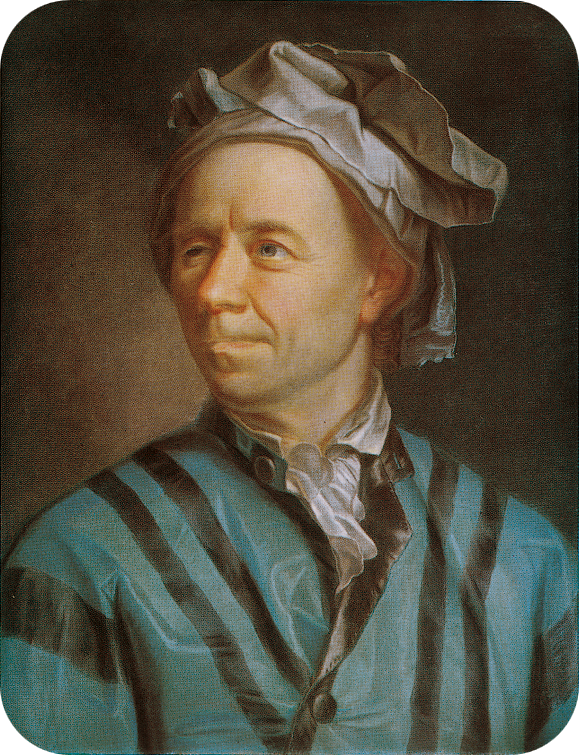
\includegraphics[width=\linewidth]{img/Euler.png}
    \caption*{Leonhard Euler}
\end{wrapfigure}

Em 1748, 101 anos após os trabalhos de Saint Vincent e de Sarasa, Leonhard Euler (1707 - 1753) calculou a base deste logaritmo natural (denominado desta maneira por Mercator). Essa base era nada mais que o número $e$ (número de Euler). A história do número de Euler é um pouco longa, faremos um breve resumo para explicar qual a sua relação com o logarítmo natural.

Em 1683, Jakob Bernoulli (1654-1705), estava estudando sobre a capitalização em juros compostos. Ele observou que ao aumentar a frequência da capitalização (diária, por hora, por minuto, etc.), o montante final aumentava, porém não tendia ao infinito, era limitado. Ele precisou estudar o seguinte limite:

\[
\lim_{n \to \infty}\left(1+\frac{1}{n}\right)^n
\]

O qual conseguiu determinar que estava entre $2$ e $3$, utilizando o teorema do binônimo de Newton.

Algumas décadas depois, em meio do século XVIII, Euler chamou este número de $e$, e conseguiu mostrar, também utilizando o teorema do binômio que

\[
e = \lim_{n \to \infty}\left(1+\frac{1}{n}\right)^n = \sum_{k=0}^{\infty}\frac{1}{k!}
\]

Mas dentro de nosso contexto, o mais interessante que Euler fez, foi mostrar que esse número seria a base do logarítmo hiperbólico (ou natural). Dessa vez, definiremos a área abaixo da hipérbole de $1$ até $a$ como sendo $A(a) = \log_{b} a$, pois agora é compreendida o conceito de base para logaritmo.

Observe que qualquer que seja a base $b$ do logaritmo hipérbolico, ele é tal que $A(b) = \log_{b} b = 1$. Faremos uma construção similar, porém diferente da proposta de Saint-Vincent.

Aproximaremos a área em $n$ retângulos, definindo $q = \sqrt[n]{b}$, então o $k$-ésimo retângulo é tal que o comprimento de sua base vale $q^{k+1} - q^k$ e sua altura é $\dfrac{1}{q^k}$, e portanto, a área de cada retângulo vale
\[
    A_k = \frac{q^{k+1}-q^k}{q^k} = q - 1
\]

\begin{figure}[H]
    \centering
    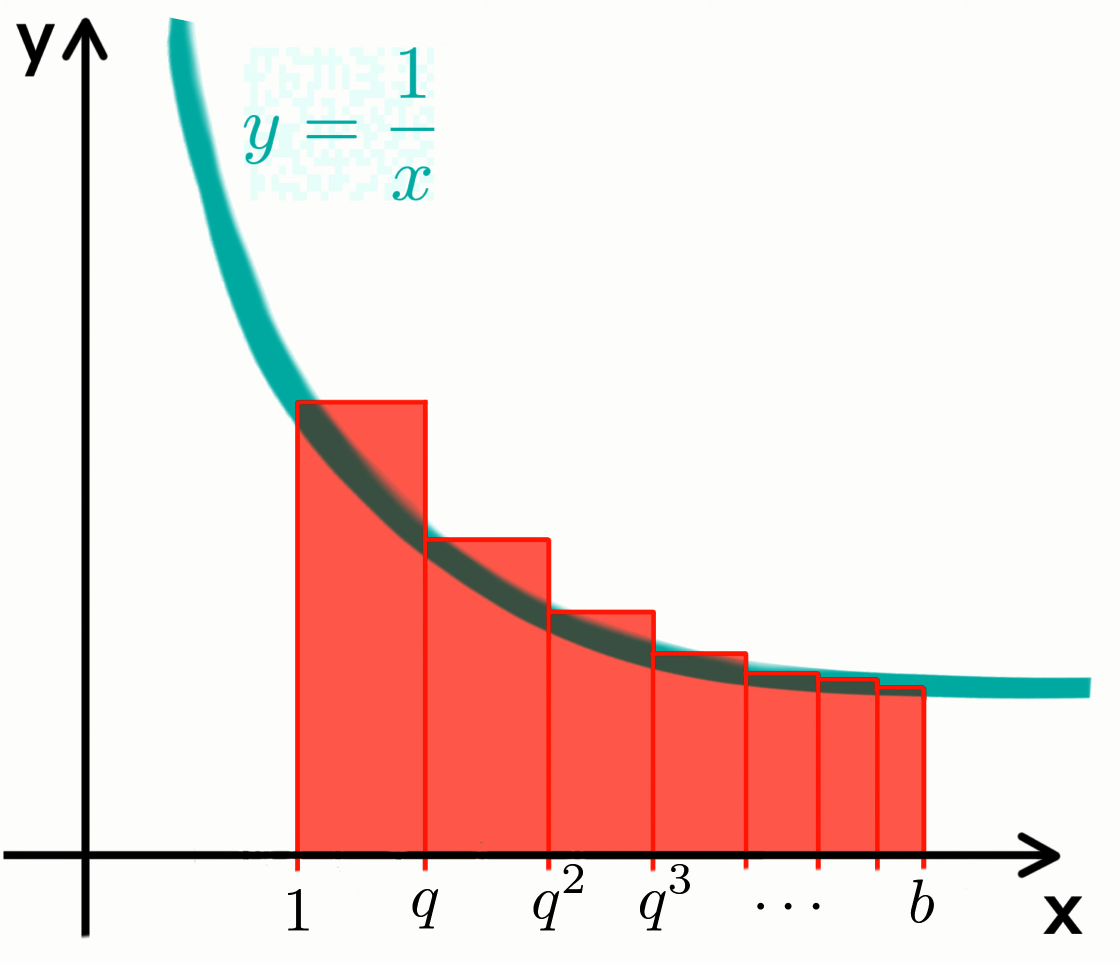
\includegraphics[width=0.5\linewidth]{img/eulerNatural.png}
    \caption{Área da Hipérbole}
    \label{fig:hiperboleeuler}
\end{figure}

Portanto, cada retângulo tem a mesma área $q - 1$, logo, a área total aproximada abaixo da hipérbole é nada mais que $A = n(q-1)$, mas sabemos que quando $n$ cresce, esse número deve tender a $1$, ou seja, $b$ deve ser tal que:

\[
    \lim_{n \to \infty} n(q - 1) = 1 \quad \text{, isto é,} \quad \lim_{n \to \infty} n(\sqrt[n]{b} - 1) = 1
\]

Esta foi a expressão que Euler obteve. É possível mostrar rigorosamente que $b$ deve ser o número $e$. Não o faremos aqui, mas daremos uma razão intuitiva:

Sabemos que deve valer o limite: $\lim_{n \to \infty} n(\sqrt[n]{b} - 1) = 1$. Então, para $n$ grande, temos que:

\[
n \left( \sqrt[n]{b} - 1 \right) \approx 1
\]

\[
\Rightarrow \sqrt[n]{b} - 1 \approx \frac{1}{n} 
\Rightarrow \sqrt[n]{b} \approx 1 + \frac{1}{n}
\]

\[
\Rightarrow b \approx \left( 1 + \frac{1}{n} \right)^n 
\xrightarrow[n \to \infty]{} e
\]

E daí, foi descoberto que $e$ era exatamente a base do logaritmo hiperbólico.